
\section{Problem definition}

\subsection{Learning a word embedding space}

In order to learn an embedding of words into vector spaces, we use the training code provided by Mikolov et. al. in word2vec\cite{word2vec}. While the original paper is short on some details, this writeup\cite{word2vec_explained} uncovers some other more esoteric portions of the paper.

\subsubsection{Skip Gram}
This model aims to predict the context given the current word. 

More specifically, we want to maximize the probability of the corpus given the following factorization:
\begin{equation}
	argmax_{\theta} \prod_{w\in text} [\prod_{c\in C(w)} p(c|w;\theta)]
\end{equation}
where $C(w)$ is the context of the word (we set the context to be 12). The above says that we want to maximize the parameters theta such that the we maximize the conditional probability of the context of a given word. 

The parameterization used to model $p(c|w;\theta) = \frac{v_{c}v_w}{\sum_{c'\in C }e^{v_{c'}v_w}}$ is a soft-max layer. 


Note that 

$v_i = W^T I(word_i) \;\;\; \forall words \;\; i$ 


is the projection of the $1-of-|V|$ representation of the word where the weights of the matrix $W$ are learned during training. 

Intuitively, the above formalization of the problem aims to maximize the likelihood of every word in the context independent of each another. The final vector representations of the words are derived from the matrix $W$



\subsubsection{Continuous Bag of Words (CBOW)}
Unlike the skip gram model, the continuous bag of words makes a bag of words assumption by summing up the projections of the context for a given word and trying to predict the word. 

We have that:
\begin{equation}
	argmax_{\theta} \prod_{w\in text} p(w|k;\theta) \text{ where } k = \sum_{c \in C(w)} v_c
\end{equation}



Given a text corpus, the code provided trains a CBOW or Skip-Gram model and produces a file where every word is assigned a vector in $\mathbb{R}^n$ where we assigned $n=300$.


\begin{figure}[h]
\centering
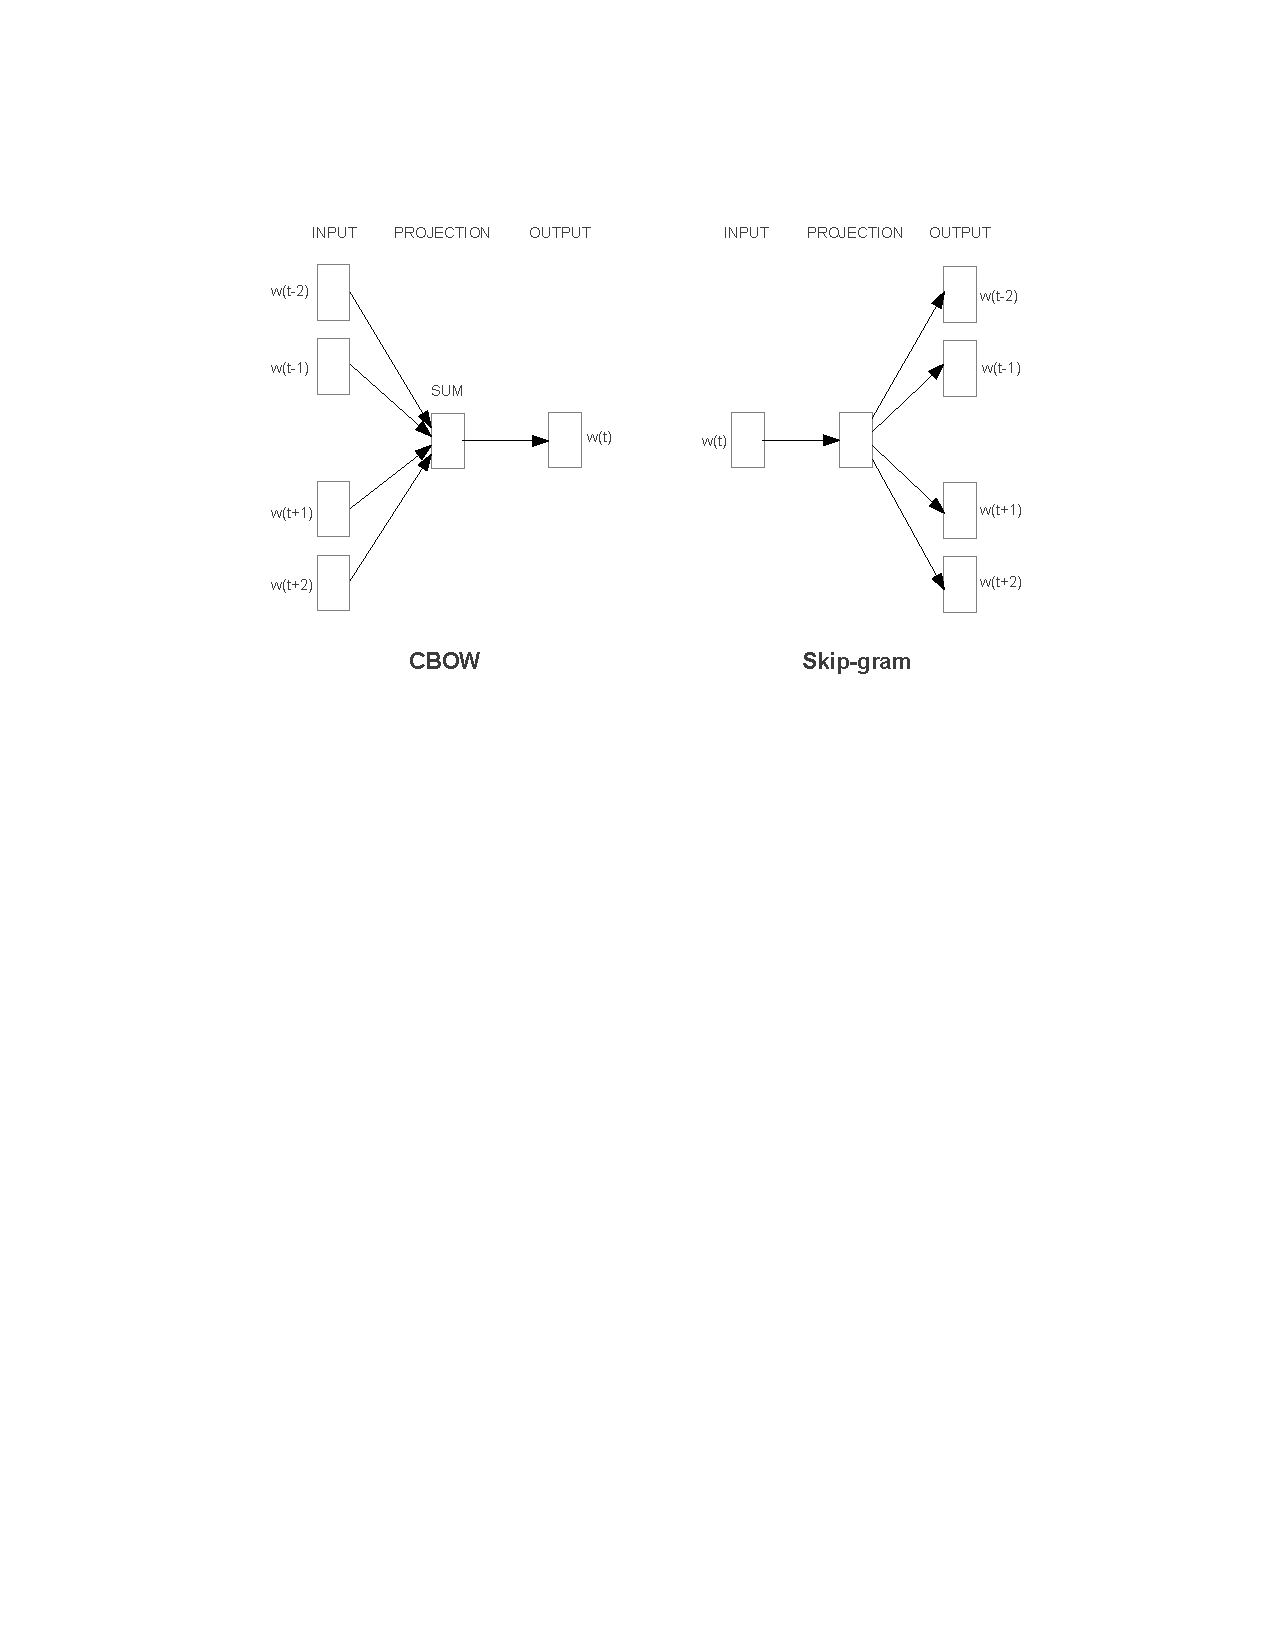
\includegraphics[width=\textwidth]{./images/model_images.pdf}
\caption{CBOW and Skip-Gram Models. Image adopted from \cite{mikolov1}}
\label{fig:top_k}
\end{figure}

\clearpage 


\subsection{Exploring properties of learned word embedding space}